The future work of probably any machine learning related implementations consists mostly of performance tuning. Sentiment analyser could be improved by considering more values during GridSearchCV tuning and also the POS tagger could considerably increase the performance. Also the process of choosing the best performing classification algorithms comparison to decide which 3 I will end up choosing for my custom analyser could be improved. I have compared their accuracy without any prior fine-tuning so it is possible some would possibly perform better with specific combination of parameters that the ones I have chosen. Another option is to build a custom training dataset from tweets talking just about web development. All these mentioned potential are still just a basic level of sentiment analysis.\\
\\
The doubt of choosing correct programming language/module/algorithm/training dataset and so on was ever-present during working on the thesis. Possible approach to tackle so many changing variables could be to create a variation points model and examine which parts of an algorithm are currently not using the best performing technology for this use-case.\\
\\
There is also another future work which could be done on top of already done work in this thesis. As the cryptocurrencies saw a big boom in the last couple of years, I thought my sentiment analyser could be used in this area as well. Without almost any tweaks, I have taken it and applied it on tweets about Bitcoin. It is very interesting to see how the sentiment changes in regards to price action. Figure \ref{fig:bitcoinSentiment} shows the sentiment change over the course of last year. There is plotted also a price development and couple of my remarks I found interesting.

\begin{figure}[H]%
    \centering
	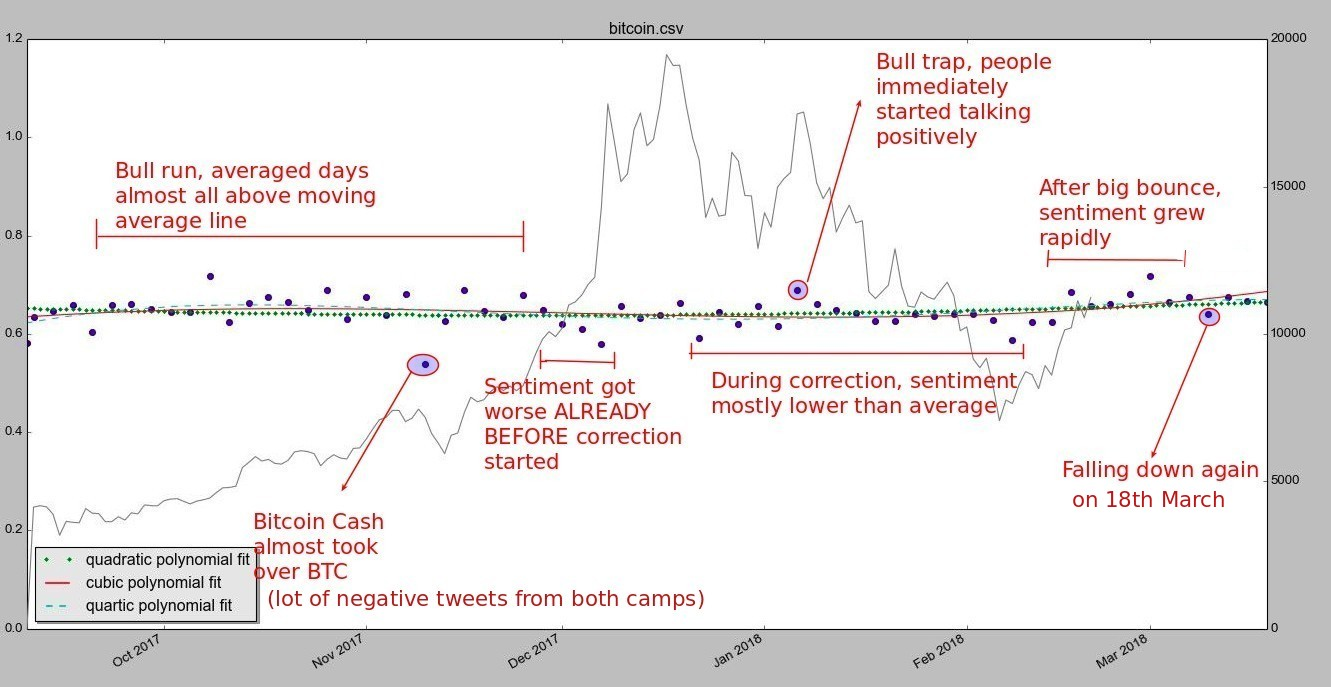
\includegraphics[width=14cm]{bitcoinSentiment.jpg}
    \caption{Change of sentiment in bitcoin tweets}%
    \label{fig:bitcoinSentiment}%
\end{figure} 

Another use I have found for my classifier during writing of this thesis was once again in cryptocurrency area. Me and my friends noticed that some small market cap coins react to good news published on their subreddits by huge value gain in just several hours. We have crawled coinmarketcap.com website which contains list of all coins with links to their respective subreddits. Then using PRAW library, we are getting all new submissions and send them to my analyser to classify them as one of 5 classes - partnership, article, exchange, roadmap and noise. These has been then continuously posted to our Slack channel as can be seen in Figure \ref{fig:toreador}. The whole process is happening in real time. For this use case, I had to change my classifier from binary to multiclass. That meant getting rid of some classifiers and adding some new ones which are able to do so, but in general, the structure of the analyser stayed the same.

\begin{figure}[H]%
    \centering
	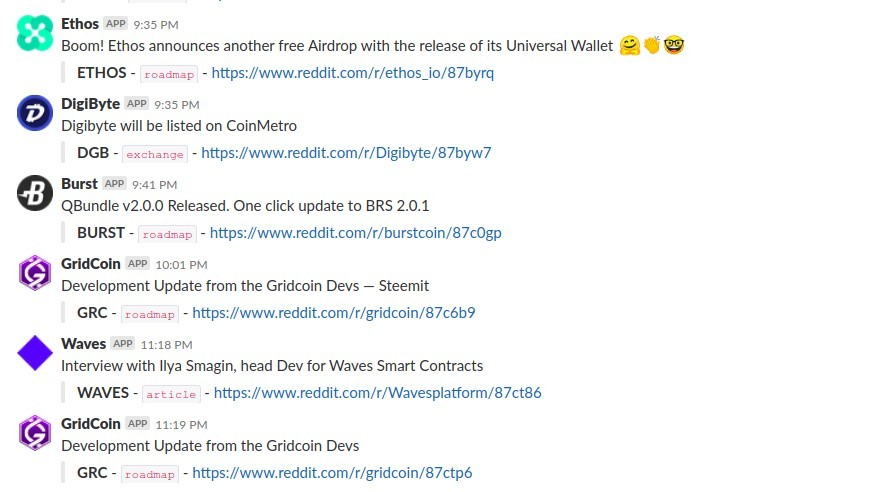
\includegraphics[width=14cm]{toreador.jpg}
    \caption{Real-time classification of cryptocurrency subreddits}%
    \label{fig:toreador}%
\end{figure} 
